%%%%%%%%%%%%%%%%%%%%%%%%%%%%%%%%%%%%%%%%%%%%%%%%%%%%%%%%%%%%%%%%%%%%%
% LaTeX Template: Project Titlepage Modified (v 0.1) by rcx
%
% Original Source: http://www.howtotex.com
% Date: February 2014
% 
% This is a title page template which be used for articles & reports.
% 
% This is the modified version of the original Latex template from
% aforementioned website.
% 
%%%%%%%%%%%%%%%%%%%%%%%%%%%%%%%%%%%%%%%%%%%%%%%%%%%%%%%%%%%%%%%%%%%%%%


\documentclass[12pt]{report}

\usepackage[portuguese]{babel}
\usepackage[a4paper]{geometry}
\usepackage[myheadings]{fullpage}
\usepackage{fancyhdr}
\usepackage{lastpage}
\usepackage{graphicx, wrapfig, subcaption, setspace, booktabs}
\usepackage[utf8]{inputenc}
\usepackage[font=small, labelfont=bf]{caption}
\usepackage{fourier}
\usepackage[protrusion=true, expansion=true]{microtype}

\usepackage{sectsty}
\usepackage{url, lipsum}
\usepackage{tgbonum}
\usepackage{hyperref}
\usepackage{listings}
\usepackage{xcolor}

\newcommand{\HRule}[1]{\rule{\linewidth}{#1}}
\onehalfspacing
\setcounter{tocdepth}{5}
\setcounter{secnumdepth}{5}


\definecolor{codegreen}{rgb}{0,0.6,0}
\definecolor{codegray}{rgb}{0.5,0.5,0.5}
\definecolor{codepurple}{rgb}{0.58,0,0.82}
\definecolor{backcolour}{rgb}{0.95,0.95,0.92}

\lstdefinestyle{mystyle}{
    backgroundcolor=\color{backcolour},   
    commentstyle=\color{codegreen},
    keywordstyle=\color{magenta},
    numberstyle=\tiny\color{codegray},
    stringstyle=\color{codepurple},
    basicstyle=\ttfamily\scriptsize,
    breakatwhitespace=false,         
    breaklines=true,                 
    captionpos=b,                    
    keepspaces=true,                 
    numbers=left,                    
    numbersep=5pt,                  
    showspaces=false,                
    showstringspaces=false,
    showtabs=false,                  
    tabsize=2
}

\lstset{style=mystyle}

\renewcommand{\contentsname}{Table of Contents}



%-------------------------------------------------------------------------------
% HEADER & FOOTER
%-------------------------------------------------------------------------------
%\pagestyle{fancy}
%\fancyhf{}
%\setlength\headheight{15pt}
%\fancyhead[L]{Student ID: 1034511}
%\fancyhead[R]{Anglia Ruskin University}
%\fancyfoot[R]{Page \thepage\ of \pageref{LastPage}}
%-------------------------------------------------------------------------------
% TITLE PAGE
%-------------------------------------------------------------------------------

\begin{document}
{
	\fontfamily{cmr}\selectfont
	\title{ 
		\normalsize 
		\textsc{}
		\\ 
		[2.0cm]
		\HRule{0.5pt} 
		\\
		\LARGE 
		\textbf{
			\uppercase{Localização Geográfica de Incêndios por Meio de Imagens}
			\HRule{2pt} 
			\\ 
			[0.5cm]
			\normalsize 
			\today 
			\vspace*{5\baselineskip}
		}
	}

\date{}

\author{
		Rafael Henrique Vareto \\ 
		Universidade Federal de Minas Gerais \\
		Departamento de Ciência da Computação
	}

\maketitle
% \tableofcontents
\newpage

%-------------------------------------------------------------------------------
% Section title formatting
\sectionfont{\scshape}
%-------------------------------------------------------------------------------

%-------------------------------------------------------------------------------
% BODY
%-------------------------------------------------------------------------------

\section*{Introdução}
% https://en.m.wikipedia.org/wiki/Correspondence_problem
O desafio proposto se refere, basicamente, ao problema de correspondência de pontos entre imagens que, embora caracterizam uma mesma cena, são obtidas de pontos de vista diferentes.
Mais especificamente, o problema da correspondência refere-se ao problema de determinar quais partes de uma imagem correspondem a quais partes de outra imagem, onde as diferenças são devidas ao movimento da câmera, ao decorrer do tempo e ao movimento dos objetos capturados nas fotos.


\section*{O Problema}
Dadas duas ou mais imagens da mesma cena 3D, tiradas de diferentes pontos de vista, o problema da correspondência refere-se à tarefa de encontrar um conjunto de pontos em uma imagem que pode ser identificado como os mesmos pontos em outra imagem. 
Para fazer isso, os pontos ou recursos em uma imagem são combinados com os pontos ou recursos correspondentes em outra imagem. 
As imagens podem ser tiradas de um ponto de vista diferente, em momentos diferentes ou com objetos na cena em movimento geral em relação às câmeras.

\begin{figure}[!h]
	\centering
	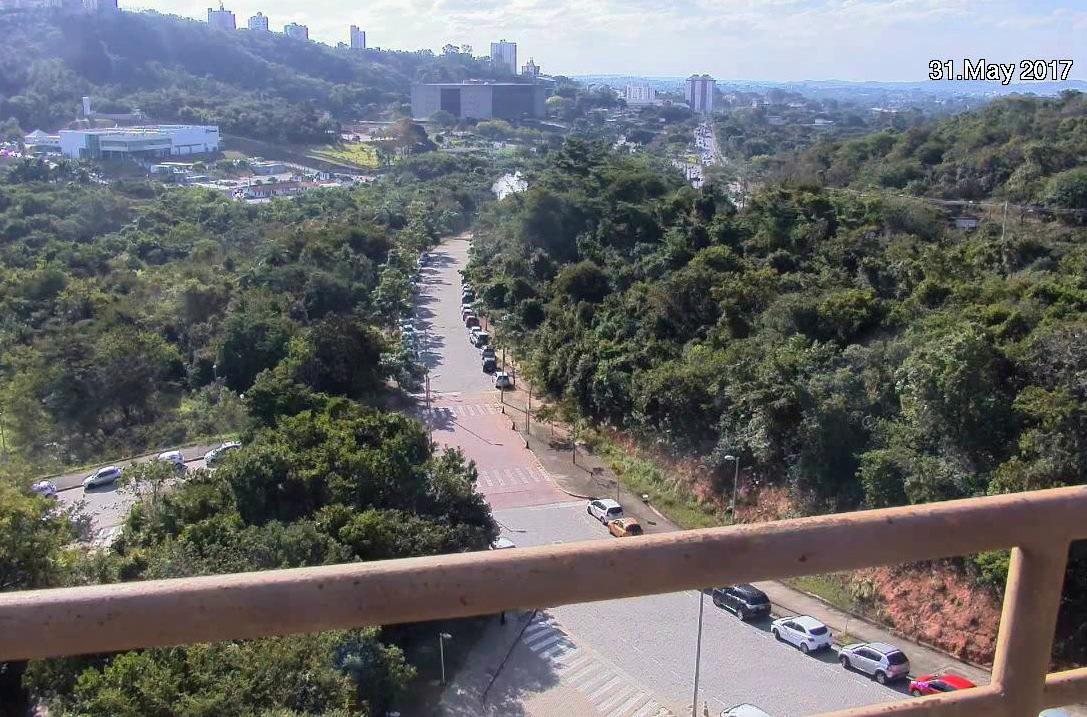
\includegraphics[width=0.85\columnwidth]{images/cemig-pic.jpg}
	\caption{Fotografia tirada do prédio da \textsc{BHTec}, na região da Pampulha em Belo Horizonte, MG.}
	\label{fig:bhtec}
\end{figure}

\noindent Assim, com as posições geográficas\footnote{Posições geográficas se referem à latitude e longitude.} da câmera $p = (-19.885087, -43.974836)$, tendo seu ponto de vista demonstrado na Figura~\ref{fig:bhtec} de resolução $1087 \times 717$, os dois objetivos do desafio são:
\begin{enumerate}
	\item Encontrar a posição geográfica do pixel $e = (412, 598)$ e avaliar o erro sabendo que a posição geográfica correspondente são as coordenadas $p_{e} = (-19.877751, -43.978796)$.
	\item Encontrar a posição geográfica do pixel $f = (510, 523)$, o qual apresenta indícios de incêndio.
\end{enumerate}

\noindent Os únicos dados disponíveis para encontrar a correspondência entre os pixeis da Figura~\ref{fig:bhtec} e as coordenadas\footnote{Coordenadas são verificadas pelo Google Maps: \url{https://goo.gl/maps/gCP1HhLgY4CpPeLK9}} são:
\begin{itemize}
	\item Pixel $a = (552, 238)$ com coordenadas $p_{a} = (-19.884362, -43.975112)$.
	\item Pixel $b = (220, 568)$ com coordenadas $p_{b} = (-19.880996, -43.978154)$.
	\item Pixel $c = (660, 613)$ com coordenadas $p_{c} = (-19.875391, -43.977202)$.
\end{itemize}

{
	\color{red}
	\noindent Vale a pena ressaltar que não foi utilizado o pixel $e = (412, 598)$ e coordenadas $p_{e} = (-19.877751, -43.978796)$ para o desafio $1$, pois isto aumentaria drasticamente a qualidade dos nossos resultados visto que queremos calcular o erro sem o conhecimento prévio da coordenada $p_{e}$.
	Por outro lado, adicionamos o pixel $e$ e sua coordenada correspondente $p_{e}$ para o desafio $2$ com o intuito de utilizar a maior quantidade possível de informação para encontrar o foco do possível incêndio.
}


\section*{Literatura}
A estimação de posição é o resultado direto da reconstrução de cenas, um dos ramos da visão computacional.
A grande maioria dos métodos existentes na literatura alcançam bom desempenho com imagens tiradas aproximadamente com o mesmo ponto de vista.
Não é o caso deste desafio, visto que coordenadas são melhor representadas por visões aéreas e espaciais.

% https://www.learnopencv.com/homography-examples-using-opencv-python-c/
Uma das formas mais eficientes de encontrar a correspondência de pontos entre imagens é através da matriz de homografia~\cite{dubrofsky2009homography}.
Uma homografia é uma transformação que mapeia os pontos em uma imagem para os pontos correspondentes na outra imagem.
Para calcular uma homografia entre duas imagens, é necessário conhecer pelo menos 4 correspondências de pontos entre as duas imagens. 
Se você tiver mais de 4 pontos correspondentes, é ainda melhor.
Essas correspondências de pontos entre imagens podem encontradas automaticamente através de algoritmos de detectam \textit{keypoints} como \textsc{sift}~\cite{lowe2004distinctive} ou \textsc{surf}~\cite{bay2006surf}.


% https://www.robots.ox.ac.uk/~vgg/hzbook/hzbook1/HZepipolar.pdf
% https://link.springer.com/content/pdf/10.1023/A:1007941100561.pdf
Também é possível encontrar a correspondência de pontos entre imagens é pela geometria epipolar~\cite{zhang1998determining}.
A geometria epipolar é um campo da visão computacional que fornece formalismo matemático e técnicas de reconstrução de cenas a partir das correspondências dos pontos de cena da imagem, sem exigir conhecimento dos parâmetros internos ou da posição relativa das câmeras.
Ela se baseia na relação entre duas imagens resultantes da projeção de uma cena através de duas câmeras em uma matriz chamada \textit{matriz fundamental}~\cite{luong1993determining}, de tamanho $3 \times 3$.
Esta matriz fundamental $F_{3 \times 3}$ encapsula a geometria intrínseca de tal forma que o ponto $x$ no mundo é representado como $x_{1}$ na primeira visualização e $x_{2}$ na segunda~\cite{hartley2004multiple} de tal forma que esses pontos satisfazem a relação $x^{T}_{2} F x_{1} = 0$.

% https://towardsdatascience.com/regression-models-with-multiple-target-variables-8baa75aacd
% https://towardsdatascience.com/understanding-random-forest-58381e0602d2
Outra forma amplamente utilizada para encontrar a relação entre duas variáveis contínuas é a regressão linear.
Aqui, procura-se encontrar um relacionamento estatístico ao invés de uma relação determinística~\cite{seber2012linear} que tende a ser utilizado quando uma variável não pode ser expressa com precisão pela outra.
Em métodos de regressão a ideia central é obter uma linha que melhor se ajuste aos dados. 
A melhor linha de ajuste é aquela para a qual o erro total de previsão (todos os pontos de dados) é o menor possível. 
Erro é a distância entre o ponto e a linha de regressão.
Para o problema de correspondência de pontos e coordenadas, é interessante utilizar métodos de regressão que suportam múltiplas variáveis dependentes para uma mesma entrada~\cite{borchani2015survey}. 
Possíveis soluções para o problema baseado em métodos de regressão seriam \textit{Random Forests}~\cite{correia2016oblique} ou Redes Neurais~\cite{liu2016multispectral}.

Uma das principais limitações da geometria epipolar gira em torno da quantidade de pontos mínimos necessários para obter uma boa correspondência entre duas imagens.
Em meu conhecimento, estes métodos precisam, obrigatoriamente, de pelo menos sete ou oito pontos em cada imagem para estabecer o relacionamento entre elas\footnote{\url{https://web.stanford.edu/class/cs231a/course_notes/03-epipolar-geometry.pdf}}.
Visto que o desafio divulgou somente três pixels ($a$, $b$ e $c$) e suas três respectivas coordenadas geográficas ($p_{a}$, $p_{b}$ e $p_{c}$), decidimos descartar esta abordagem e focar em estratégias de homografa e métodos de regressão que suportem múltiplas variáveis dependentes.
Embora métodos de regressão não estabeleçam uma quantidade mínima de amostras, é recomendado utilizar uma quantidade considerável para uma boa generalização do método.


\section*{Estratégia 1: Random Forests}
% https://towardsdatascience.com/random-forest-and-its-implementation-71824ced454f
\textit{Random Forests}~\cite{breiman2001random} é um algoritmo de aprendizado supervisionado capaz de executar tarefas de regressão e classificação com o uso de várias árvores de decisão.
É uma técnica baseada em Bagging~\cite{breiman1996bagging} que aprende diversos métodos de regressão (modelos) em paralelo sem que haja qualquer interação entre eles.
Cada modelo representa uma característica diferente do conjunto de dados pois subconjuntos dos dados são amostrados de forma aleatória e permite uma melhor compreensão da variância e do viés do conjunto de dados.
Ele opera construindo uma infinidade de árvores de decisão no momento do treinamento e retorna a previsão média (regressão) das árvores individuais.
Ao final, ele combina a predição realizada por cada modelo e faz a agregação através de votos ou simplesmente a média de todos eles.
Uma das principais vantagens do \textit{Random Forests} é o fato de ser bastante preciso, fornecendo estimativas de quais variáveis são importantes para a regressão.


% convert img25.jpg img24.jpg img23.jpg img22.jpg img21.jpg -append result-sprite.jpg
% https://stackoverflow.com/questions/20075087/how-to-merge-images-in-command-line

% \newpage
% \noindent\textbf{Código Fonte}
\subsection*{Código Fonte}
\begin{lstlisting}[language=Python, caption=Código-fonte com Random Forests implementado para a obtenção de valores aproximados para as coordenadas.]
from geopy.distance import geodesic
from scipy.spatial import distance
from sklearn.ensemble import RandomForestRegressor

trainX = [
    [552, 238], # a (red)
    [220, 568], # b (red)
    [660, 613], # c (red)

    # [548, 598], # Usiminas (green)
    # [489, 595], # Usiminas (blue)
    # [611,  18], # BHTec prox (blue)
    # [146, 224], # BHTec descida (blue)
]

trainY = [
    [-19.884362, -43.975112], # a (red)
    [-19.880996, -43.978154], # b (red)
    [-19.875391, -43.977202], # c (red)

    # [-19.877094, -43.978037], # Usiminas (green)
    # [-19.877851, -43.978243], # Usiminas (blue)
    # [-19.884660, -43.974987], # BHTec prox (blue)
    # [-19.884490, -43.975472], # BHTec descida (blue)
]

validX = [[412,598]]
validY = [[-19.877751,-43.978796]]
probeF = [[510,523]]

regr = RandomForestRegressor(max_depth=20, random_state=3, n_estimators=200)
regr.fit(trainX, trainY)

predY = regr.predict(validX)
euc_error = distance.euclidean(validY, predY)
met_error = geodesic(validY, predY).meters

print(validY, predY, euc_error, met_error)
\end{lstlisting}

Com a implementação de \textit{Random Forests} disponível na biblioteca \textit{Scikit Learn}\footnote{\url{https://scikit-learn.org/stable/modules/generated/sklearn.ensemble.RandomForestRegressor.html}}, configuramos os seguintes parâmetros empiricamente:
\texttt{max\_depth} define a profundidade máxima da árvore. 
\texttt{n\_estimators} determina o número de árvores na floresta.
\texttt{random\_state} é a semente usada pelo gerador de números aleatórios.
A saída do código fonte contido em \textbf{Listing 1} imprime a coordenada esperada, a coordenada predita, a distância euclidiana das coordenadas, e a distância em metros das coordenadas.


\section*{Estratégia 2: Homografia}
Uma homografia é uma transformação em perspectiva de um plano, ou seja, uma re-projeção de um plano de uma câmera para uma visualização diferente, sujeita a alterações na translação (posição) e rotação (orientação) da câmera~\cite{detone2016deep}.
As transformações de perspectiva mapeiam pontos 3D em planos de imagem 2D usando a matriz de transformação que incorpora as características da câmera: distância focal, centro óptico e os parâmetros extrínsecos (rotação, translação).
Para reprojetar um ponto de uma câmera para outra, teríamos que projetar inversamente o ponto $x$ da imagem no sistema de coordenadas do mundo e, em seguida, reprojetar no novo plano de imagem com a câmera traduzida e girada, para obter a homografia.

\subsection*{Código Fonte}
\begin{lstlisting}[language=Python, caption=Código-fonte com Homografia implementado para a obtenção de valores aproximados para as coordenadas.]
from geopy.distance import geodesic
from scipy.spatial import distance
from sklearn.ensemble import RandomForestRegressor

import cv2 as cv
import numpy as np

pixelsPhoto = np.array([
    [552, 238], # a (red)
    [220, 568], # b (red)
    [660, 613], # c (red)

    # [247, 522], # Aglomerado1 (green)
    # [548, 598], # Usiminas (green)
    # [489, 595], # Usiminas (blue)
    # [611,  18], # BHTec prox (blue)
    # [459, 396], # BHTec med (blue)
    # [468, 484], # BHTec longe (blue)
    # [146, 224], # BHTec descida (blue)
])

coords = np.array([
    [-19.884362, -43.975112], # a (red)
    [-19.880996, -43.978154], # b (red)
    [-19.875391, -43.977202], # c (red)

    # [-19.881952, -43.977276], # Aglomerado1 (green)
    # [-19.877094, -43.978037], # Usiminas (green)
    # [-19.877851, -43.978243], # Usiminas (blue)
    # [-19.884660, -43.974987], # BHTec prox (blue)
    # [-19.883896, -43.975428], # BHTec med (blue)
    # [-19.882713, -43.975915], # BHTec longe (blue)
    # [-19.884490, -43.975472], # BHTec descida (blue)
])

homo, status = cv.findHomography(pixelsPhoto, coords)
Ephoto = [[412, 598, 1]]
Ecoord = [[-19.877751, -43.978796]]

result = np.dot(homo, np.transpose(Ephoto))
normed =  (1/result[2]) * result

euc_ds = np.sqrt((normed[0] - Ecoord[0][0])**2 + (normed[1] - Ecoord[0][1])**2)
met_error = geodesic(Ecoord, normed).meters
print(Ecoord, np.transpose(normed[0:2]), euc_ds[0], met_error)
\end{lstlisting}

Com a implementação da Matriz de Homografia disponível na biblioteca \textit{OpenCV}\footnote{\url{https://docs.opencv.org/master/d9/dab/tutorial_homography.html}}, fornecemos os pontos referente aos pixeis da foto e suas respectivas coordenadas geográficas (latitude e longitude) a fim de relacionar a transformação entre dois possíveis planos.
Semelhantemente à estratégia anterior, a saída do código fonte contido em \textbf{Listing 2} retorna a coordenada esperada, a coordenada predita, a distância euclidiana das coordenadas, e a distância em metros das coordenadas.


\section*{Experimentos}
Com preocupações práticas como memória e tempo do processamento de lado, é difícil imaginar nenhuma situação onde ter dados de treinamento mais representativos leve a um resultado pior. 
Assim, aumentar o tamanho do conjunto de dados tende a reduzir correlações espúrias, diminuir a variância dos dados e melhorar o desempenho de métodos de regressão.
A possibilidade de discrepâncias faz parte do que torna importante ter uma grande quantidade de amostras.
Em outras palavras, aumentar o tamanho da amostra comumente evita estatísticas enganosas, principalmente se houver alguma irregularidade (\textit{outliers}) em algumas amostras.
O tamanho da amostra está diretamente relacionado à margem de erro de uma estatística ou à precisão com que ela pode ser calculada.
Por esta razão, \textbf{decidimos fazer experimentos adicionais inserindo novos pontos ao desafio}.
De fato, realizamos uma avaliação partindo dos três pontos fornecidos inicialmente pelo desafio e depois vamos adicionando gradativamente novos pontos.
A Figure~\ref{fig:bhtec2} exibe os pontos originais em vermelho e os pontos adicionais em azul.

\begin{figure}[!h]
	\centering
	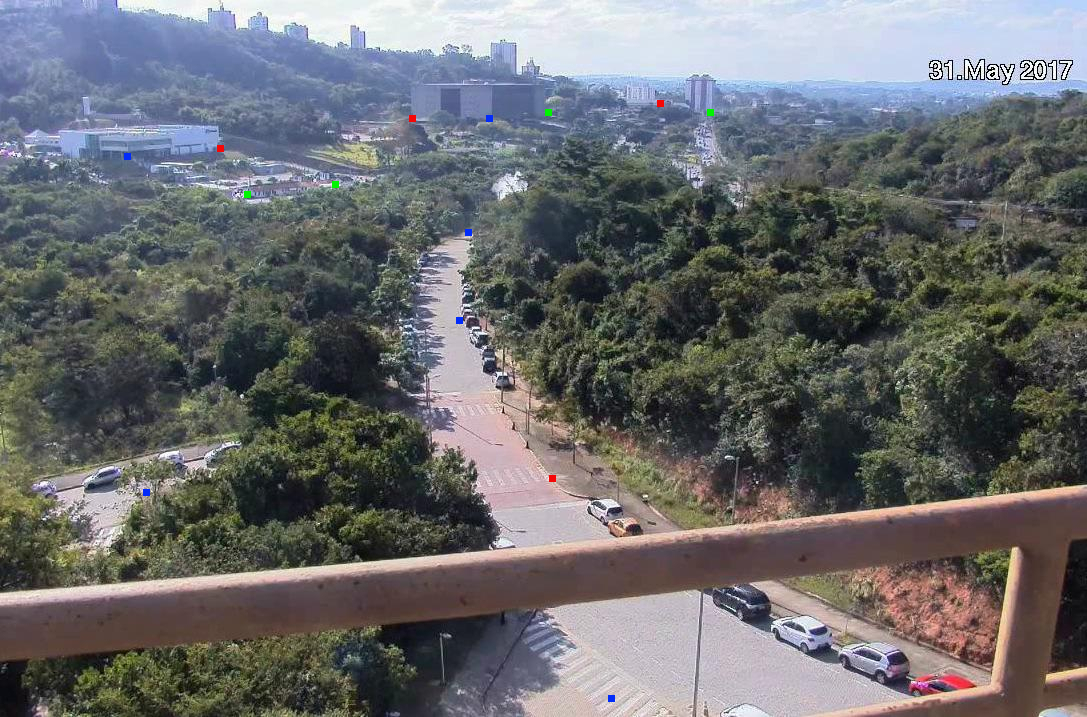
\includegraphics[width=0.85\columnwidth]{images/cemig-pic-2.jpg}
	\caption{Fotografia tirada do prédio da \textsc{BHTec}, na região da Pampulha em Belo Horizonte, e contendo os pontos demarcados. Em vermelho estão os pontos fornecidos pelos organizadores do desafio e em verde e azul se encontram os pontos adicionais.}
	\label{fig:bhtec2}
\end{figure}

\newpage

\begin{table}[!h]
	\centering
	\scriptsize
    \begin{tabular}{c|rr|rr}
		\textbf{Pontos} & \multicolumn{2}{c|}{\textbf{Random Forest}}                & \multicolumn{2}{c}{\textbf{Homografia}}                     \\ \hline
		Métrica         & Euclidiana                   & \multicolumn{1}{c|}{Metros} & \multicolumn{1}{c}{Euclidiana} & \multicolumn{1}{c}{Metros} \\ \hline\hline
		3               & 0.002084                     & \textbf{223.938}            & 0.015892                       & 1758.382                   \\
		4               & 0.000987                     & \textbf{103.495}            & 0.003088                       & 341.900                    \\
		5               & 0.000729                     & \textbf{76.676}             & 0.000842                       & 89.979                     \\
		6               & 0.000709                     & \textbf{74.449}             & 0.000742                       & 79.881                     \\
		7               & 0.000693                     & 72.674                      & 0.000549                       & \textbf{59.022}            \\
		8               & 0.000725                     & 76.039                      & 0.000288                       & \textbf{30.623}            \\
		9               & 0.000777                     & 81.791                      & 0.000177                       & \textbf{18.660}            \\
		10              & 0.000833                     & 87.523                      & 0.000141                       & \textbf{15.009}            \\ \hline     
    \end{tabular}
    \caption{Resultados (erro) obtidos em cada uma das estratégias para o desafio 1}
    \label{tab:results1}
\end{table}

Na Tabela~\ref{tab:results1} apresentamos os erros obtidos com as duas estratégias.
Apresentamos tanto a distância euclidiana quanto a distância em metros de cada uma das coordenadas reais para as coordenatas preditas pelo modelo.
Quando é empregado somente três pontos (pixeis $a$, $b$ e $c$) e suas respectivas posições geográficas (coordenadas $p_{a}$, $p_{b}$, $p_{c}$) é alcançada uma distância de aproximadamente 223 e 1758 metros empregando \textit{Random Forests} e Homografia, respectivamente.
Perceba que ao adicionar mais pontos e coordenadas, a acurácia de ambos os métodos cresce consideravelmente, resultando numa menor taxa de erro.
Como mencionado anteriormente, esse comportamento é esperado visto que adicionamos amostras e, consequentemente, aumentamos a capacidade de generalização das duas abordagens. 
Assim, com pontos adicionais, alcançamos a distância de cerca de 72 e 15 metros empregando \textit{Random Forests} e Homografia, respectivamente.

\begin{table}[!h]
	\centering
	\scriptsize
	\begin{tabular}{c|cc|cc}
		\textbf{Coord.} & \multicolumn{2}{c|}{\textbf{Desafio 1}}            & \multicolumn{2}{c}{\textbf{Desafio 2}}         \\ \hline
		Pontos               & Random Forests        & Homografia            & Random Forests        & Homografia            \\ \hline \hline
		3                    & -19.879141,-43.977242 & -19.893563,-43.980389 & -19.880094,-43.977404 & -19.878460,-43.977367 \\
		4                    & -19.877645,-43.977814 & -19.880839,-43.978741 & -19.879404,-43.977768 & -19.883478,-43.975773 \\
		5                    & -19.877561,-43.978091 & -19.878240,-43.978110 & -19.879410,-43.978081 & -19.887209,-43.975063 \\
		6                    & -19.877613,-43.978100 & -19.878265,-43.978260 & -19.879324,-43.977977 & -19.886716,-43.975103 \\
		7                    & -19.877726,-43.978102 & -19.878113,-43.978382 & -19.879072,-43.978070 & -19.885775,-43.975281 \\
		8                    & -19.877798,-43.978071 & -19.877894,-43.978545 & -19.879075,-43.978091 & -19.885516,-43.975222 \\
		9                    & -19.877976,-43.978052 & -19.877798,-43.978624 & -19.881488,-43.976608 & -19.885377,-43.975218 \\
		10                   & -19.877918,-43.977979 & -19.877810,-43.978667 & -19.881690,-43.976844 & -19.885181,-43.975246 \\ \hline
	\end{tabular}
    \caption{Coordenadas obtidas em cada uma das estratégias para os desafios 1 e 2}
    \label{tab:results2}
\end{table}

Na Tabela~\ref{tab:results2} apresentamos as coordenadas obtidas em ambos os desafios com as duas estratégas implementadas.
Vale a pena ressaltar que para os desafios 1 e 2, não utilizamos dados referentes ao pixel $e$ e sua respectiva coordenada $p_{e}$.
Por outro lado, adicionamos pontos anotados manualmente levando em conta o ponto de vista da fotografa dada e as coordenadas obtidas pelo Google Maps. %\footnote{\url{www.google.com/maps}}. 
Ou seja, esses pontos podem estar sujetos a ruídos humanos e podem gerar mais entropia nos dados do que, de fato, melhorar os resultados.
Isto provavelmente justifica o aumento da taxa de erro na estratégia baseada em \textit{Random Forests} quando sete pontos/coordenadas ou mais são adicionados.


\section*{Conclusão} 

Em ambos os desafios propostos foi possível avaliar algumas estratégias difundidas na literatura que visam resolver o problema de correspondência entre pontos.
A utilização de métodos estatísticos (\textit{Random Forests}) de regressão e algébricos (Homografia) permitiram encontrar coordenadas geográficas relativamente aproximadas de suas localizações originais.
Também constatamos que ao adicionar mais pontos e coordenadas aos métodos, mesmo que manualmente anotadas, há um ganho na acurácia dos mesmos com a diminuição da distância (erro) entre a posição genuína e a predita.
Todos os resultados se encontram nas tabelas.
Foram utilizadas duas bibliotecas da linguagem Python: \texttt{OpenCV 4.0.0} e \texttt{Scikit Learn 0.21.3}.
Os códigos também estão em anexo no e-mail e podem ser utilizados para conferência dos resultados obtidos.



%-------------------------------------------------------------------------------
% REFERENCES
%-------------------------------------------------------------------------------
\bibliographystyle{unsrt}
\bibliography{references}

}
\end{document}


